\documentclass{report}
\usepackage[utf8]{inputenc}
\usepackage{textgreek}
\usepackage{gensymb}
\usepackage{graphicx}
\usepackage{listings}
\usepackage{amsmath}
\graphicspath{ {pdf/} }



\begin{document}
\chapter{Simulation of X-Ray Pump Probe Experiments}

\section{Intensity Position Monitor}
At the X-Ray Pump Probe (XPP) beamline of SLAC National Accelerator Laboratory's LCLS, there are two beam monitors upstream of the sample position.
They are bespoke single shot intensity position monitors (IPM).
The first, IPM\textsubscript{2} is upstream of attenuator.
The second is IPM\textsubscript{3} is closer to the sample position, but suffers from less intense readings on the whole.
The IPM detectors both consist of four 10 cm square diodes (Figure \ref{ipm}).
Photons from the incident X-Ray beam are scattered by an amorphous silicon nitride (Si\textsubscript{3}N\textsubscript{4}) membrane.
Backscattered X-rays are collected on the detector panels and read out once per shot as the four intensity values $I_T, I_R, I_B, I_L$. 
The beam flux is then proportional to the sum of the panel readings, $I\propto \sum_{i\in T,R,B,L}I_i$. 
Furthermore, the position of them beam can be constrained by the panel readings as $Xpos\propto \frac{I_R-I_L} {I_R + I_L}$ and $Ypos\propto \frac{I_T-I_B} {I_T + I_B}$. 
    
\subsection{Estimating Si\textsubscript{3}N\textsubscript{4} Backscatter}
The X-ray beam incident on the silicon nitride film is polarized in the X plane. 
The polarization of the incident beam indicates that the scattering to the horizontal detectors will predominate. 
In order to estimate the relative scattering to each of the panels, we can use the polarized expression of the Klein-Nishina formula \cite{Klein1929-ic}. 
The major contributions to scattering according to Klein and Nishina can be broken down into elastic and inelastic contributions. 
The differential scattering cross section of the elastic Thompson component of the Klein-Nishina equation is given as \cite{Namito1993-tk}
\begin{equation}
\label{thompson}
\bigg( \frac {d\sigma}{d\Omega} \bigg)_T = r_0^2(1 - \sin^2\theta \cos^2 \phi)
\end{equation}
wherein $r_0$ is the classical radius of an electron. 
The angle \texttheta\ is the angle between the incident beam wavevector and the scattered beam wavevector. 
\textphi\ is the angle between the scattered beam wavevector and the incident beam polarization vector. 
The differential inelastic portion of the backscatter is given by \cite{Namito1993-tk}
 
\begin{equation}
\label{compton}
\bigg( \frac {d\sigma}{d\Omega} \bigg)_C = \frac {1} {2} r_0^2 \bigg(\frac{k}{k_0}\bigg)^2\bigg(\frac {k} {k_0} + \frac {k_0} {k} - 2 \sin^2 \theta \cos^2 \phi \bigg).
\end{equation}

The scattered beam energy, k, for inelastic Compton scattering is a function of scattering angle and incident photon energy \cite{Heitler1954-vq}.
\begin{equation}
k = \frac {k_0 \mu} {\mu + k_0 (1 - \cos \theta)}
\end{equation}

$\mu = mc^2$ is the rest mass energy of an electron. 
These equations may be integrated to estimate the relative intensities of photons scattered by a free electron onto the detector panels. 
\begin{equation}
I_P = \int_{P} \bigg[  \bigg( \frac {d\sigma}{d\Omega} \bigg)_C 
+ \bigg( \frac {d\sigma}{d\Omega} \bigg)_T \bigg]
\end{equation}

They may also be augmented by the atomic form factors and scattering factors to estimate intensities for specific elements. 

\begin{equation}
I_P = \int_{P} \bigg[  S \bigg( \frac {\sin ( \theta/2 )}{\lambda}, Z \bigg) \bigg( \frac {d\sigma}{d\Omega} \bigg)_C 
+ F^2 \bigg( \frac {\sin ( \theta/2 )}{\lambda}, Z \bigg) \bigg( \frac {d\sigma}{d\Omega} \bigg)_T \bigg]
\end{equation}

However, the geometry of the detector system makes it difficult to integrate over the panel in spherical coordinates. Therefore, it is prudent to convert the spherical coordinates to cartesian coordinates in the detector system as in Figure \ref{ipm}. This can be achieved by the relationships

\begin{equation}
\begin{align*}
\theta &= \pi - \tan^{-1} {\bigg( \frac {\sqrt{(x-xpos)^2 + (y-ypos)^2}} {l} \bigg)} \\
\phi   &= \tan^{-1} \bigg(\frac {y - ypos} {x - xpos} \bigg)
\end{align*}
\end{equation}



\begin{figure}
\centering
\includegraphics[width=0.8\textwidth]{ipm.pdf}
\caption{Geometry of the Intensity Position Monitor}
\label{ipm}
The IPM detector has four panels, here refered to as Top, Right, Bottom, and Left. The panels are 10 mm squares. The inner edge of the panels are found 10 mm from the centroid of the detector diode system. The X-ray beam position here is denoted by Xpos, Ypos in the cartesian detector coordinate system.  
\end{figure}

\begin{figure}
\centering
\includegraphics[width=0.8\textwidth]{theta.pdf}
\caption{Scattering off silicon nitride membrane to detector diode}
Downstream of the detector by a distance z=l, is a silicon nitride film. 
At XPP, we believe that l is essentially 20 mm and that the film is 4 \textmu m thick. 
Photons scattered by the film are detected on the IPM panels. 
The scattering angle, \texttheta, is defined with respect to the forward scattering direction. 
Therefore, backscattered photons, as we detect here, are \textpi-\texttheta  degrees from the Z axis. 
The backscattered photon shown above is the special case wherein \textphi=90 degrees. 
However, in the general case, theta determines a circle in which the scattered photon can hit the detector system. 
The particular angle along that circle is given by \textphi. 
\end{figure}

\begin{figure}
\centering
\includegraphics[width=0.8\textwidth]{phi.pdf}
\caption{Relation between cartesian detector system and scattering angles \texttheta\ and \textphi}
\end{figure}

\section{Model for For Observed Reflection Intensities}
In order to generate, realistic "observations" of Bragg peak intensities, $I_h$, several factors must be considered. 
Chiefly, the reflection intensity is proportional to the square of the structure factor amplitude. 
However, the squared structure factor amplitude must be modified by several factors. 

\begin{equation}
I_h \propto F_h^2pfI_o
\end{equation}

The partiality, $p$, of a given observation is the fraction of that reflection which was observed on the detector. 
In X-FEL experiments, the X-ray pulses are too brief to move the detector during data collection. 
Therefore, all detector readouts only contain a portion of the 3-D reciprocal space volume of each reflection. 
For the moment, simulated partialities are simply drawn from a normal distribution. 
This approach finds some justification in the knowledge that Serial Femtosecond Crystallography essentially works by assuming partialities are sampled from a guassian. 
In addition to the partiality of the reflection, which is an intrinsic consequence of the crystal's mosaicity and alignment, the fraction of the incoming photons incident on the crystal needs to be taken into account. 
This is particularly important given that positional fluctions in the X-ray beam are often on the order of $\frac {1} {10}$ to $\frac {1} {5}$ of the linear dimension of the crystal. 
To compute the fraction of light incident on the crystal, $f$, we need to integrate over the X-ray beam intensity distribution. 
Here, we simply model the beam as a bivariate normal, $\mathcal{N}(\mu, \Sigma)$ with mean values, $\mu=\{xpos, ypos\}$ covriance matrix

\begin{equation}
\Sigma = 
\[
\begin{bmatrix}
    \sigma_x^2 & 0 \\
    0 & \sigma_y^2 \\
\end{bmatrix}.
\]
\end{equation}

Where the variances correspond to the linear aspect of the x-ray beam in the x and y dimensions. Generally, these numbers are in the 10s of microns. 
To compute f, we simply integrate $\mathcal{N}$ over the surface area of the crystal. 

\begin{equation}
\begin{align*}
f &= \int_A \frac {1} {2\pi \sigma_x \sigma_y} e^{-\frac {1} {2} \big[ \frac {(x - xpos)^2}{\sigma_x^2} + \frac {(y - ypos)^2}{\sigma_y^2} \big]} \\
f &= \frac {1} {4} \bigg[ \bigg( Erf (\frac {xmin - xpos} {\sqrt {2} \sigma_x}) - Erf (\frac {xmax - xpos} {\sqrt {2} \sigma_y)} )\bigg)   \bigg( Erf ( \frac {ymin - ypos} {\sqrt {2} \sigma_y}) - Erf (\frac {ymax - ypos} {\sqrt {2} \sigma_y}) \bigg)  \bigg]
\end{align*}
\end{equation}

\section{Command Line Arguments for Data Simulator}
The data simulator in Gammastimator has been designed to be reasonably flexible with sane defaults. 
The only thing that necessarilly be provided by the end user are on and off structure factor amplitudes in CNS file format.
CNS was chosen, because it is the most sane plain text format that Phenix understands. 
The command signature for simulate.py is

\begin{lstlisting}
python simulate.py [options] Foff Fon out
\end{lstlisting}

\bibliographystyle{plain}
\bibliography{references}

\end{document}
